% Chapter X

\chapter{Diseño del Protocolo CWC} % Chapter title

\label{ch:diseno_cwc} % For referencing the chapter elsewhere, use \autoref{ch:name} 

%----------------------------------------------------------------------------------------

\section{Estructura de los Mensajes}
\label{sec:estructura_protocolo_cwc}

El protocolo de comunicación se basará en XML para realizar el envío y recepción de mensajes entre el servidor, los clientes y las cachés. En el presente apartado se definirá los mensajes que se intercambiarán y sus respuestas.

Cualquier mensaje que se envíe siempre tendrá tres componentes, que servirán como identificador de éste:

\begin{figure}[h]
  \centering
    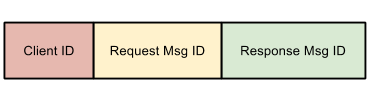
\includegraphics[scale=0.75]{gfx/EstructuraMensajeCWC}
  \caption{Estructura de un mensaje}
  \label{EstructuraMensajeCWC}
\end{figure}


En la figura \ref{EstructuraMensajeCWC} se observan los componentes del mensaje, los cuales son:

\begin{enumerate}
\item El identificador único del cliente en el sistema, este es generado cuando un cliente entra a formar parte de la comunidad, en el caso del servidor su identificador único es 0. En algunos mensajes se utilizará un identificador por defecto (-1) este significará que hay un nuevo cliente que desea convertirse en un miembro de la comunidad pero aun no tiene su identificador único.

\item Request Message Id: Este es el número del mensaje al que se esté respondiendo, cuando se encuentre el caso que no se esté respondiendo a ningún mensaje se introducirá un número negativo lo cual indicara que se está iniciando una comunicación.

\item Response Message Id: Este es el número del mensaje que estamos enviando, este número se genera como un aleatorio entre 1 y 10000, en algunos casos el mensaje no necesita respuesta entonces se introduce un número negativo.
\end{enumerate}

%------------------------------------------------

\section{Operaciones del Protocolo}

En el presente apartado se definirán las operaciones necesarias para el funcionamiento del protocolo CWC. Aquí de detallará tanto valores de entrada, como de salida y además la estructura esperada. 

%------------------------------------------------

\subsection{ACK}

Este mensaje es una confirmación. Además puede ser enviado por cualquiera de las partes involucradas en la comunicación: Servidor o Cliente. Éste tiene la siguiente estructura:

\begin{lstlisting}[language=XML,caption=Mensaje ACK]
<ack clientid="XXXX" requestid="XXXX" responseid="-1"> </ack>
\end{lstlisting}

\begin{description}
\item[Respuesta] No necesita respuesta.
\end{description}

%----------------------------------------------------------------------------------------

\subsection{GetClientId}

Este mensaje se utiliza cuando un nuevo CWCClient quiere formar parte de la comunidad. La estructura del mensaje es:

\begin{lstlisting}[language=XML,caption=Mensaje GetClientId]
<getClientId clientid="-1" requestid="-1" responseid="XXXX"> 
</getClientId>
\end{lstlisting}


Como se puede observar el clientId es -1 ya que es un cliente nuevo, el requestId es -1 ya que no se está respondiendo a nadie y el responseid es un numero aleatorio entre 1 y 10000. 

\begin{description}
\item[Respuesta] La Respuesta esperada por parte del servidor es:
\end{description}

 \begin{lstlisting}[language=XML,caption=Mensaje de Respuesta GetClientId]
<getClientId clientid="0" requestid="XXXX" responseid="YYYY"> 
	<client> ZZZZ </client>
</getClientId>
\end{lstlisting}

Para terminar la comunicación se espera por parte del cliente un ACK con su nuevo clientId.

\subsection{UpdateMembership}

Este mensaje se utiliza para establecer el tipo de membresía, recursos que se están prestando a la caché y tipo de administración. La primera vez que se utiliza, lo que se busca es crear la membresía, lo usos subsecuentes son básicamente para actualizar la información. La estructura del mensaje debería ser:

\begin{lstlisting}[language=XML,caption=Mensaje de UpdateMembership]
<UpdateMembership clientid="XXXX" requestid="-1" responseid="YYYY"> 
	<type> ZZZZ </type>
	<manage> ZZZZ </manage>
	<disk> ZZZZ </disk>
	<mem> ZZZZ </mem>
	<upload> ZZZZ </upload>
</UpdateMembership>
\end{lstlisting}

Los valores que pueden tomar estas variables son:

\begin{itemize}
\item \textbf{type}: 1 = Voluntaria, 2 = Involuntaria
\item \textbf{manage}: 1 = Atendida, 2 = desatendida, 3 = Administrada por servidor
\item \textbf{disk}: En MB un número mayor o igual a 100
\item \textbf{mem}: En MB un número mayor o igual a 100
\item \textbf{upload}: En KB un número mayor o igual 128
\end{itemize}

\begin{description}
\item[Respuesta] Se espera como respuesta un ACK por parte del servidor.
\end{description}

\subsection{GetObjectInfo}
Este mensaje se utiliza para obtener la información de un objeto cacheable. La estructura es:

\begin{lstlisting}[language=XML,caption=Mensaje de GetObjectInfo]
<GetObjectInfo clientid="XXXX" requestid="-1" responseid="YYYY"> 
	<objectId> ZZZZ </objectId>
	<objectLocation> ZZZZ </objectLocation>
</GetObjectInfo>
\end{lstlisting}

Los valores que pueden tomar estas variables son:

\begin{itemize}
\item \textbf{objectId}: El identificador único del objeto.
\item \textbf{objectLocation}: El URI relativo del objeto cacheable.
\end{itemize}

Es posible que se incluya solo uno o ambos.

\begin{description}
\item[Respuesta] La Respuesta esperada por parte del servidor es:
\end{description}

\begin{lstlisting}[language=XML,caption=Mensaje de Respuesta de GetObjectInfo]
<response clientid="0" requestid="XXXX" responseid="YYYY"> 
	<checksum> ZZZZ </checksum>
	<id> ZZZZ </id>
	<location> ZZZZ </location>
	<size> ZZZZ </size>
	<expdate> ZZZZ </expdate>
</response>
\end{lstlisting}

Lo valores que retorna son:

\begin{itemize}
\item \textbf{checksum}:  El Checksum del archivo
\item \textbf{id}: El identificador del objeto
\item \textbf{location}: URI relativo donde se encuentra el objeto.
\item \textbf{size}: Tamaño del archivo en megabytes
\item \textbf{expdate}: Fecha de expiración.
\end{itemize}


La respuesta esperada por parte del cliente es un ACK.

\subsection{ModifyObject}
Este mensaje es enviado por el servidor, en este caso se ha realizado un cambio del lado del servidor que debe ser propagado hacia los clientes. La estructura del mensaje es:

\begin{lstlisting}[language=XML,caption=Mensaje de ModifyObject]
<ModifyObject clientid="0" requestid="XXXX" responseid="YYYY"> 
	<checksum> ZZZZ </checksum>
	<id> ZZZZ </id>
	<location> ZZZZ </location>
	<size> ZZZZ </size>
	<expdate> ZZZZ </expdate>
	<type> ZZZZ </type>
</ModifyObject>
\end{lstlisting}

La única diferencia con el anterior es el type, el cual especifica el tipo de modificación que se está realizando, 1 significa una modificación soft la cual no necesita actualizar el archivo y cualquier otra cosa es una modificación hard lo que implica que hay que deshabilitar el archivo y volverlo a cargar.

\begin{description}
\item[Respuesta] La respuesta esperada por parte del cliente es un ACK.
\end{description}

\subsection{Enable-Disable Object}

En este caso el mensaje se utiliza para habilitar o deshabilitar un objeto que se encuentra en la caché. Este mensaje puede ser enviado tanto por el servidor como por el cliente. La estructura del mensaje es:

\begin{lstlisting}[language=XML,caption=Mensaje de EnableObject]
<EnableObject clientid="XXXX" requestid="-1" responseid="YYYY"> 
	<objectId> ZZZZ </objectId>
</EnableObject>
\end{lstlisting}

Se envía el identificador del objeto, si el objeto esta Enable se cambia a Disable o viceversa  y se espera un ACK de parte de la otra parte.

\begin{description}
\item[Respuesta] La respuesta esperada por parte del cliente o servidor, según corresponda, es un ACK.
\end{description}

\subsection{DeleteObject}
Este mensaje es utilizado ya sea por los clientes o por el servidor, cuando un objeto se borra en alguno de los dos. La estructura del mensaje es:

\begin{lstlisting}[language=XML,caption=Mensaje de DeleteObject]
<DeleteObject clientid="XXXX" requestid="-1" responseid="YYYY"> 
	<objectId> ZZZZ </objectId>
</DeleteObject>
\end{lstlisting}

Se envía el identificador del objeto y se registra el borrado, en el caso del cliente borra el objeto de la cache, en el caso del servidor borra la relación entre la cache y el objeto.

\begin{description}
\item[Respuesta] La respuesta esperada por parte del cliente o servidor, según corresponda, es un ACK.
\end{description}

\subsection{GetMemberStatus}
\label{GetMemberStatus} 
Este mensaje es utilizado para solicitar el estado de un miembro de la caché (no del servidor), se puede ejecutar tanto por el servidor como por cualquier miembro de la caché. La estructura del mensaje es:

\begin{lstlisting}[language=XML,caption=Mensaje de GetMemberStatus]
<GetMemberStatus clientid="XXXX" requestid="-1" responseid="YYYY"> 
	<memberId> ZZZZ </memberId>
</GetMemberStatus>
\end{lstlisting}

\begin{description}
\item[Respuesta] Se envía el memberId que es igual al clientId, se espera la siguiente respuesta:
\end{description}

\begin{lstlisting}[language=XML,caption=Mensaje de Respuesta de GetMemberStatus]
<response clientid="0" requestid="XXXX" responseid="YYYY"> 
	<status> ZZZZ </status>
</response>
\end{lstlisting}

El status puede tomar los siguientes valores 0 = desconocido, 1 = activo, 2 = no-activo, 3 = offline y 4 = online.

Se espera un ACK por parte de quien solicitó el status.

\subsection{ChangeMemberStatus}
Este mensaje es utilizado para cambiar el status de un miembro de la cache, este solo puede ser ejecutado por parte del servidor hacia cualquiera de los clientes o  por parte del cliente hacia el servidor para cambiar su estatus. La estructura del mensaje es:

\begin{lstlisting}[language=XML,caption=Mensaje de ChangeMemberStatus]
<ChangeMemberStatus clientid="0" requestid="XXXX" responseid="YYYY"> 
	<memberId> ZZZZ </memberId>
	<status> ZZZZ </status>
</ChangeMemberStatus>
\end{lstlisting}


El status puede tomar cualquier valor de la operación definida en \ref{GetMemberStatus}. 


\begin{description}
\item[Respuesta] La respuesta esperada por parte del cliente es un ACK.
\end{description}

\subsection{GetListOfFiles}

Este mensaje se utiliza ya sea para pedir una lista de archivos a un cliente con su respectivo checksum o para solicitar una lista de archivo que debería tener un cliente en su caché con su respectivo checksum. La estructura de este mensaje es:

\begin{lstlisting}[language=XML,caption=Mensaje de GetListOfFiles]
<GetListOfFiles clientid="0" requestid="XXXX" responseid="YYYY"> 
	<clientId> ZZZZ </clientId>
</GetListOfFiles>
\end{lstlisting}

\begin{description}
\item[Respuesta] La Respuesta esperada por parte del cliente es:
\end{description}

\begin{lstlisting}[language=XML,caption=Mensaje de Respuesta de GetListOfFiles]
<response clientid="0" requestid="XXXX" responseid="YYYY"> 
	<file objectId="ZZZZ" checksum="ZZZZ"> </file>
	<file objectId="ZZZZ" checksum="ZZZZ"> </file>
	<file objectId="ZZZZ" checksum="ZZZZ"> </file>
</response>
\end{lstlisting}

Se espera un ACK por parte de quien recibe la lista de archivos.

\subsection{GetStats}
Se ejecuta por parte del servidor, para obtener las estadísticas de una de las cachés, la estructura del mensaje es:

\begin{lstlisting}[language=XML,caption=Mensaje de GetStats]
<GetStats clientid="XXXX" requestid="-1" responseid="YYYY"> 
	<clientId> ZZZZ </clientId>
</GetStats>
\end{lstlisting}



\begin{description}
\item[Respuesta] La Respuesta esperada por parte del cliente es:
\end{description}

\begin{lstlisting}[language=XML,caption=Mensaje de Respuesta de GetStats]
<response clientid="0" requestid="XXXX" responseid="YYYY"> 
	<maxupload> ZZZZ </maxupload>
	<minupload> ZZZZ </minupload>
	<maxclients> ZZZZ </maxclients>
	<currentclients> ZZZZ </currentclients>
</response>
\end{lstlisting}

Se envía la máxima velocidad de transferencia, la mínima velocidad de trasferencia, máxima cantidad de clientes simultaneemos y clientes actuales.

Se espera un ACK por parte de quien recibe las estadísticas.

\subsection{SendStats}

En algunos casos las estadísticas son enviadas por el mismo cliente, en este caso la estructura del mensaje es:

\begin{lstlisting}[language=XML,caption=Mensaje de SendStats]
<SendStats clientid="0" requestid="XXXX" responseid="YYYY"> 
	<maxupload> ZZZZ </maxupload>
	<minupload> ZZZZ </minupload>
	<maxclients> ZZZZ </maxclients>
	<currentclients> ZZZZ </currentclients>
</SendStats>
\end{lstlisting}

\begin{description}
\item[Respuesta] La Respuesta esperada por parte del servidor es un ACK.
\end{description}

\subsection{GetTopCachesbyObject}

Este mensaje es enviado por los clientes, para solicitar el top de cachés que pueden servir un objeto. El formato del mensaje es:

\begin{lstlisting}[language=XML,caption=Mensaje de GetTopCachesbyObject]
<GetTopCachesbyObject clientid="0" requestid="XXXX" responseid="YYYY"> 
	<objectId> ZZZZ </objectId>
</GetTopCachesbyObject>
\end{lstlisting}


\begin{description}
\item[Respuesta] La Respuesta esperada por parte del servidor es:
\end{description}

\begin{lstlisting}[language=XML,caption=Mensaje de Respuesta de GetTopCachesbyObject]
<response clientid="0" requestid="XXXX" responseid="YYYY"> 
	<cache clientId="ZZZZ" URL="ZZZZ"> </cache>
	<cache clientId="ZZZZ" URL="ZZZZ"> </cache>
	<cache clientId="ZZZZ" URL="ZZZZ"> </cache>
</response>
\end{lstlisting}


Se espera un ACK por parte del cliente que recibió esta lista.

\subsection{GetConfParams}
Este también es únicamente ejecutado por el cliente, se utiliza para tomar la configuración del sistema, hay varios parámetros que pueden cambiar, este mensaje se utiliza para obtener estos cambios. La estructura del mensaje es:

\begin{lstlisting}[language=XML,caption=Mensaje de GetConfParams]
<GetConfParams clientid="0" requestid="XXXX" responseid="YYYY"> 
</GetConfParams>
\end{lstlisting}


\begin{description}
\item[Respuesta] La Respuesta esperada por parte del servidor es:
\end{description}

\begin{lstlisting}[language=XML,caption=Mensaje de Respuesta de GetConfParams]
<response clientid="0" requestid="XXXX" responseid="YYYY"> 
	<param paramId="ZZZZ"> </param>
	<param paramId="ZZZZ"> </param>
	<param paramId="ZZZZ"> </param>
</response>
\end{lstlisting}


Se espera un ACK por parte de quien recibe la lista de parámetros.

\subsection{IsAlive}

Este mensaje se utiliza para saber si algún miembro del sistema está vivo. La estructura del mensaje es:

\begin{lstlisting}[language=XML,caption=Mensaje de IsAlive]
<IsAlive clientid="XXXX" requestid="-1" responseid="YYYY"> 
</IsAlive>
\end{lstlisting}

\begin{description}
\item[Respuesta] Para este mensaje es espera un ACK por parte de la cache representada por clientId.
\end{description}

\section{Seguimiento de los miembros conectados}

Es de suma importancia saber si alguno de los miembros de la CWC se encuentra bien, para esto se deberá estar revisando que los miembros estén en línea, para lograrlo, se seguirá:

\begin{enumerate}
\item El servidor tendrá una estampa de tiempo para cada cache, la cual indicara la última vez que se recibió un mensaje por parte de esta.
\item Cada cache tendrá una estampa de tiempo del servidor que indicara la última vez que este envió un mensaje.
\item Existirá un parámetro configurable llamado "tiempo sin respuesta", el cual establece cuanto tiempo debe pasar después de que se recibió un mensaje para preocuparse.
\item Cada vez que se recibe un mensaje por parte de alguna caché o el servidor, se establece esta estampa a la hora en la cual se recibió el mensaje.
\item Se estará revisando periódicamente si alguna estampa ya es lo suficientemente antigua como para que el tiempo actual menos la estampa del último mensaje se mayor o igual al "tiempo sin respuesta".
\item Si ha pasado más tiempo del establecido por "tiempo sin respuesta", se envía un mensaje de IsAlive.
\item Si no se recibe respuesta después de tres intentos se establece que esa caché o servidor esta caído.
\item En el caso de una cache, se seguirá revisando periódicamente en tiempos no menores a "tiempo sin respuesta" hasta que se descubra que está arriba.
\item En el caso del servidor se actualizará la caché como offline y se esperaré a que ésta se comunique.
\end{enumerate}

\section{Recuperación de fallas}
Cuando se presenta una falla, se puede dar ya sea en el lado del servidor como del lado de alguno de los clientes, el protocolo que se seguirá es:

\subsection{¿Cómo descubrir una falla?}
Para descubrir una falla se deben de dar las siguientes condiciones:
\begin{enumerate}
\item En el caso del servidor perder contacto con todas las caches y con Internet (una implica a la otra).
\item En el caso de un cliente perder la conexión con el servidor o con Internet (una implica a la otra). 
\end{enumerate}

\subsection{Falla del Servidor}
Una falla se puede dar por muchas razones, no es nuestro objetivo estudiarlas, el caso es que se pueden dar de dos tipos:

\begin{itemize}
\item Se pierda información volátil: Esto quiere decir que el servidor por ejemplo se apague, lo cual hace que la información que estaba en memoria y no se había enviado a disco o a base de datos mediante un flush, se perdió.
\item Que no se pierda información volátil: Por ejemplo que se pierda la conexión a Internet o que se apague voluntariamente el servidor entonces se cortan las funciones de red.
\end{itemize}

En cualquier caso este es el protocolo:

\begin{enumerate}
\item Si es sin pérdida de información volátil: Se debe hacer un flush inmediatamente.
\item Una vez que nos hallamos recuperado de la falla, en este caso nos damos cuenta de que fue así ya que tenemos comunicación con las caches y con Internet, dejamos a todas las cache en un estado desactivadas.
\item Cargamos la información a memoria.
\item Esperamos la petición por estado, cuando el estado es desactivado se procede a revisar la consistencia.
\item Esperamos que recibir los mensajes por parte de las caches, que ante esta eventualidad, enviaran mensajes GetListOfFiles.
\item Esperamos hasta que las caches envíen un cambio (ChangeStatus) de estado a en línea.
\item Esperamos que se repita esto las veces que sean necesarias.
\item Después de que las caches estén en línea, retomaran los mensajes donde habían quedado (recordemos se guarda el último mensaje enviado, si no se recibe respuesta se declara que está abajo el servidor hasta que responda y se retoma la comunicación en el último mensaje enviado)
\end{enumerate}

\subsection{Falla un Cliente}
En este caso la cache por alguna razón perdió comunicación y el servidor la marco como inactiva, cuando se recupera la comunicación lo primero que se solicita es el estado de la cache, este recibirá un desactivada entonces pedirá los archivos para revisar la consistencia, cuando todo esté correcto solicitara volver a estar en estado en línea y seguirá la comunicación como estaba anteriormente.
Para reconstruir el DGET, el cliente deberá evaluar la cantidad de partes descargadas y solicitar la lista de caches disponibles al servidor para retomar la descarga.

\section{Implementación del Modelo de Consistencia}
Como se mencionó anteriormente el modelo de consistencia no es tan complejo debido a que solo un actor es el que modifica los objetos que se incluyen en la caché, este actor es el CWCServer, el modelo de consistencia bastará con:

\begin{itemize}
\item Si se modifica un objeto en el servidor, este ejecutara un ModifyObject hacia todas las caches que tienen copias de este objeto, si es un cambio de archivo tamaño, entre otros. Decidirá si es necesario eliminar el archivo y volver a solicitarlo.
\item Las caches estarán revisando periódicamente, la consistencia, esto quiere decir que solicitara al servidor el Checksum de los archivos que tiene en su cache, lo calculara y lo comparara.
\item Si hay algo extraño, simplemente solicita que se envé el archivo de nuevo, si todo está bien pues no hay ningún problema.
\item Después de una falla se revisa la consistencia, esto aplica para todas las caches en el caso de que sea una falla de servidor o para la cache que fallo.
\end{itemize}